\documentclass[a4paper, 12pt]{article}
\usepackage[utf8]{inputenc}
\usepackage[portuguese]{babel}

\usepackage{mathptmx}
\usepackage{enumitem}
\usepackage{amsmath}

% Margins
\usepackage{geometry}
\geometry{left=30mm,right=20mm,%
bindingoffset=0mm, top=30mm,bottom=20mm,includefoot}

% Images
\usepackage{graphicx}
\graphicspath{ {./images/} }

% Title font size
\usepackage{titlesec}
\titleformat*{\section}{\bfseries}

% Indent first sentence of a paragraph
\usepackage{indentfirst}

% highlight code
\usepackage{listings}

% Page numbers at bottom right
\usepackage{fancyhdr}
\pagestyle{fancy}
\fancyhf{}
\renewcommand{\headrulewidth}{0pt}
\rfoot{\thepage}

% 1.5 line spacing (yes, 1.25 is actually 1.5)
\fontsize{10}{12}
\linespread{1.50}
\fontfamily{ptm}
\selectfont

% Fix vspacing for section titles
\let\oldsection\section
\renewcommand{\section}[1]{{\vspace{20pt}\oldsection*{#1}\vspace{-10pt}}}

% Indent size
\setlength\parindent{10mm}

% Jump 20pt
\newcommand{\jump}[1]{{\vspace{20pt}}}

\newenvironment{leftquote}[1][]
{
    \hspace{30pt} #1
    \vspace{20pt}
    \fontsize{10}{10}\selectfont
    \begin{flushright}
    \begin{minipage}{120mm}
}
{
    \end{minipage}
    \end{flushright}
    \par
    \vspace{20pt}
}

\newcommand{\tmp}{}

\newenvironment{container}[3]
{
    \renewcommand{\tmp}{#3} %gambiarra
    
    \begin{center}
    \begin{minipage}{#1}
    \centering
    #2
}
{
    \raggedright
    {\footnotesize \tmp}
    \end{minipage}
    \end{center}
}

\begin{document}
	
	% Remove page number
	\clearpage
	\thispagestyle{empty}
	
	\begin{bfseries}
		\begin{center}
			
			
\includegraphics[scale=0.45]{ufc.png} \\
			\vspace{-4pt} 
			UNIVERSIDADE FEDERAL DO CEARÁ \\
			\vspace{4pt} 
			CENTRO DE TECNOLOGIA \\
			\vspace{4pt} 
			DEPARTAMENTO DE TELEINFORMÁTICA \\
			\vspace{4pt}
			\vspace{4pt}
			SEMESTRE 2025.1 \\
			
			
			\vspace*{\fill}
			\textbf{Relatório dos Homeworks de Álgebra Linear}
			\vspace*{\fill}
			
		\end{center}
		
		\begin{itemize}[leftmargin=*]
			\setlength{\itemsep}{0pt}
			\item[] ALUNO: Ruan Pereira Alves
			\item[] MATRÍCULA: 569551
		\end{itemize}
		
	\end{bfseries}
	\newpage
	
	\section{Homework 01 linear}
	
	Em álgebra linear, podemos verificar como podemos fazer a resolução de sistemas lineares de forma um pouco mais dinâmica, e especialmente como é possível realizar operações utilizando vetores coluna, o que permite interpretar as operações utilizando as colunas do sistema, mantendo o formato $Ax = b$. 
	
	Um espaço vetorial é constituído de vetores que possuem as operações de adição de vetores e multiplicação de escalares, e que alguns axiomas devem ser seguidos para que as operações ocorram. O maior exemplo de um espaço vetorial é o espaço $R^n$, que pode possuir $n$ dimensões.
	
	Um subespaço seria apenas um subconjunto de vetores dentro de um espaço vetorial, vide exemplo $R^3$.
	
	Após isso, precisamos verificar se um dado conjunto de vetores possui independência linear, ou seja se os vetores só possuem uma forma de serem zerados, sendo "forçados" a serem zero. Em outras palavras, o espaço nulo da matriz A com os vetores só possui o vetor zero.
	
	Com essa independência, podemos assim gerar um espaço com base no conjunto de vetores, em que as combinações destes vetores criam o espaço vetorial, ou seja baseado em operações entre esses vetores. O espaço vai consistir de todas as possíveis combinações lineares do conjunto de vetores. 
	
	Uma base seria uma sequência de vetores que justamente possui as duas propriedades mencionadas acima. Para qualquer espaço, o número de vetores-base é uma propriedade do próprio espaço, ou seja para qualquer número de vetores-base de um espaço, o mesmo número de vetores é contido dentro do espaço, o que nos traz o conceito de dimensão. 
	
	Para a verificação de um vetor arbitrário em um subespaço definido, é necessário realizar as operações vetoriais com os vetores-base do subespaço, buscando montar o vetor arbitrário a partir dos vetores-base, ou seja criando um sistema linear e o resolvendo. Se houver solução, o vetor pertence. 
	
	Assim, foi possível realizar o desenvolvimento da atividade, vide o código a seguir: 
	
	\begin{lstlisting}
		import numpy as np
		A = np.array([[1, 2, 3],
		[4, 5, 6],
		[7, 8, 9]])
		
		print("hello\n", A)
		
		det_A = np.linalg.det(A)
		print("det A =", det_A)
		
		B = np.array([[3, 2, 1],
		[0, 0, 0],
		[0, 0, 0]])
		
		print(A + B)
		
		C = A * 2
		print(C)
		
		r = np.linalg.matrix_rank(A)
		print(r)
		
		base = np.eye(3)
		
		arb = np.array([2, 2, 1])
	\end{lstlisting}
	
	\section{Homework 02 linear}
	
	Para o item 2, precisamos primeiro entender o que seria um problema de Least Squares, que é basicamente uma combinação linear dos parâmetros da equação, que quando derivados, devem assumir formato $x = (A^T A)^{-1} A^T y$, com isso, temos que:
	
	$$
	x_{\text{opt}} = \arg \min_{x} \| y - Ax \|_2^2
	$$
	
	Primeiro, definimos a função de custo $J(x)$ e a reescrevemos usando a propriedade de que a norma ao quadrado de um vetor $v$ é igual ao produto escalar $v^T v$.
	
	\begin{align*}
		J(x) &= \| y - Ax \|_2^2 \\
		&= (y - Ax)^T (y - Ax)
	\end{align*}
	
	Usando a propriedade da transposta de um produto, $(AB)^T = B^T A^T$, expandimos a expressão:
	
	\begin{align*}
		J(x) &= (y^T - (Ax)^T) (y - Ax) \\
		&= (y^T - x^T A^T) (y - Ax)
	\end{align*}
	
	Agora, distribuímos os termos (multiplicação de matrizes):
	
	\begin{align*}
		J(x) &= y^T y - y^T(Ax) - (x^T A^T)y + (x^T A^T)(Ax) \\
		&= y^T y - y^T Ax - x^T A^T y + x^T A^T Ax
	\end{align*}
	
	Note que os termos $y^T Ax$ e $x^T A^T y$ são escalares (matrizes $1 \times 1$). Um escalar é igual à sua própria transposta, portanto $(y^T Ax)^T = x^T A^T y$. Isso significa que os dois termos do meio são idênticos. Podemos combiná-los:
	$$
	J(x) = y^T y - 2x^T A^T y + x^T A^T Ax
	$$
	
	O próximo passo é calcular o gradiente de $J(x)$ em relação ao vetor $x$, denotado por $\nabla_x J(x)$. Para isso, usamos as seguintes identidades do cálculo matricial:
	\begin{enumerate}
		\item $\nabla_x (c) = 0$ (o gradiente de uma constante é o vetor nulo).
		\item $\nabla_x (x^T b) = b$ (para um vetor $b$ constante).
		\item $\nabla_x (x^T B x) = 2Bx$ (para uma matriz $B$ simétrica). A matriz $A^T A$ é sempre simétrica.
	\end{enumerate}
	
	Aplicando essas regras à nossa função de custo:
	
	\begin{align*}
		\nabla_x J(x) &= \nabla_x (y^T y - 2x^T A^T y + x^T (A^T A) x) \\
		&= \nabla_x(y^T y) - \nabla_x(2x^T A^T y) + \nabla_x(x^T (A^T A) x) \\
		&= 0 - 2A^T y + 2(A^T A)x
	\end{align*}
	
	O gradiente de $J(x)$ é, portanto:
	$$
	\nabla_x J(x) = 2(A^T Ax - A^T y)
	$$
	
	No ponto de mínimo, o gradiente da função deve ser o vetor nulo. Como a função de custo é convexa, este ponto será um mínimo global 
	\begin{align*}
		& \nabla_x J(x) = 0 \\
		& 2(A^T Ax - A^T y) = 0 \\
		& A^T Ax - A^T y = 0
	\end{align*}
	
	Isso nos leva a
	$$
	A^T Ax = A^T y
	$$
	
	O passo final é isolar o vetor $x$. Assumindo que a matriz $A^T A$ é invertível (o que ocorre se as colunas da matriz $A$ forem linearmente independentes), podemos pré-multiplicar ambos os lados pela inversa $(A^T A)^{-1}$:
	
	\begin{align*}
		& (A^T A)^{-1} (A^T Ax) = (A^T A)^{-1} (A^T y) \\
		& I x = (A^T A)^{-1} (A^T y) \\
		& x = (A^T A)^{-1} A^T y
	\end{align*}
	
	onde $I$ é a matriz identidade.
	
	A solução $x_{\text{opt}}$ que minimiza a soma dos quadrados dos erros é dada pela fórmula das equações normais:
	
	$$
	x_{\text{opt}} = (A^T A)^{-1} A^T y.
	$$
	
	\begin{lstlisting}
		SNR_db = np.arange(0, 31, 5)
		iter_max = 100
		error = np.zeros((len(SNR_db), iter_max))
		
		for snr_idx, snr_val in enumerate(SNR_db):
		for iter in range(iter_max):
		x = np.random.randn(5, 1) + 1j*np.random.randn(5, 1)
		A = np.random.randn(10, 5) + 1j*np.random.randn(10, 5)
		y = A @ x
		
		snr_linear = 10**(snr_val/10)
		var_noise = (np.linalg.norm(y)**2) / snr_linear
		noise = np.sqrt(var_noise/2) * (np.random.randn(10, 1) + 1j*np.random.randn(10, 1))
		
		y_noisy = y + noise
		x_est = np.linalg.pinv(A) @ y_noisy
		
		nmse = np.linalg.norm(y - A @ x_est)**2 / np.linalg.norm(y)**2
		error[snr_idx, iter] = nmse
		
		mean_error = 10 * np.log10(np.mean(error, axis=1))
		
		plt.figure(figsize=(10, 6))
		plt.plot(SNR_db, mean_error, '-o', label='Least Squares')
		plt.ylabel('NMSE($\\hat{y}$) in dB')
		plt.xlabel('SNR (dB)')
		plt.legend(loc='best')
		plt.grid(True)
		plt.title('Least Squares Performance')
		plt.show()
	\end{lstlisting}
	
	\section{Homework 03 linear}
	
	Para o problema 1, a Decomposição de Valores Singulares (SVD) é uma técnica fundamental de fatoração de matrizes que decompõe qualquer matriz em três componentes: um conjunto de vetores singulares à esquerda, uma matriz diagonal de valores singulares e um conjunto de vetores singulares à direita. Essa decomposição é particularmente poderosa para o processamento de imagens, pois ordena naturalmente os valores singulares do maior para o menor, onde os maiores valores singulares contêm as informações mais significativas sobre a imagem.
	
	Quando aplicada à reconstrução de imagens, a SVD nos permite aproximar a matriz da imagem original, mantendo apenas os valores singulares mais significativos e descartando os menores. Esse processo é conhecido como SVD truncada. A ideia principal é que a energia da imagem (medida pela soma dos valores singulares ao quadrado) se concentra nos primeiros valores singulares. Ao selecionar uma classificação de truncamento apropriada (J), podemos reconstruir a imagem com perda mínima de qualidade, reduzindo significativamente a quantidade de dados necessária para representá-la.
	
	Para implementar isso, primeiro carregamos a imagem e a convertemos em uma matriz de valores de pixel. Em seguida, calculamos a SVD dessa matriz, que nos fornece os valores singulares e seus vetores singulares correspondentes. Os valores singulares são analisados para determinar quanta energia cada um contribui para a energia total da imagem. Normalmente, escolhemos uma classificação de truncamento $J$ tal que a energia cumulativa dos primeiros $J$ valores singulares exceda um certo limite, como $95\%$ da energia total. A imagem reconstruída é então formada pela multiplicação dos primeiros $J$ vetores singulares à esquerda, dos primeiros $J$ valores singulares e dos primeiros $J$ vetores singulares à direita.
	
	Na presença de ruído, a SVD também atua como uma ferramenta de redução de ruído. Quando o ruído é adicionado à imagem, ele tende a afetar os valores singulares menores de forma mais significativa. Ao truncar a SVD, filtramos efetivamente o ruído, visto que o ruído é frequentemente associado aos valores singulares menores. O desempenho dessa redução de ruído depende da relação sinal-ruído (SNR). Valores de SNR mais altos resultam em melhor qualidade de reconstrução, pois o ruído é menos dominante. Por outro lado, em valores de SNR mais baixos, o ruído pode obscurecer os valores singulares menores, dificultando a separação do sinal do ruído.
	
	Assim, inicialmente fazendo a reconstrução a partir da decomposição SVD truncada, obtemos a seguinte imagem:
	
	\begin{figure}[!h]
		\centering
		\includegraphics[width=0.7\linewidth]{images/recon_J.pdf}
		\caption{Imagem reconstruída a partir da operação SVD truncada.}
		\label{fig:wave}
	\end{figure}
	
	Analisando a matriz que forma a imagem, podemos observar o perfil de energia da imagem em relação com os valores singulares da matriz, para assim escolher o número de autovalores descartados.
	
	\begin{figure}[!h]
		\centering
		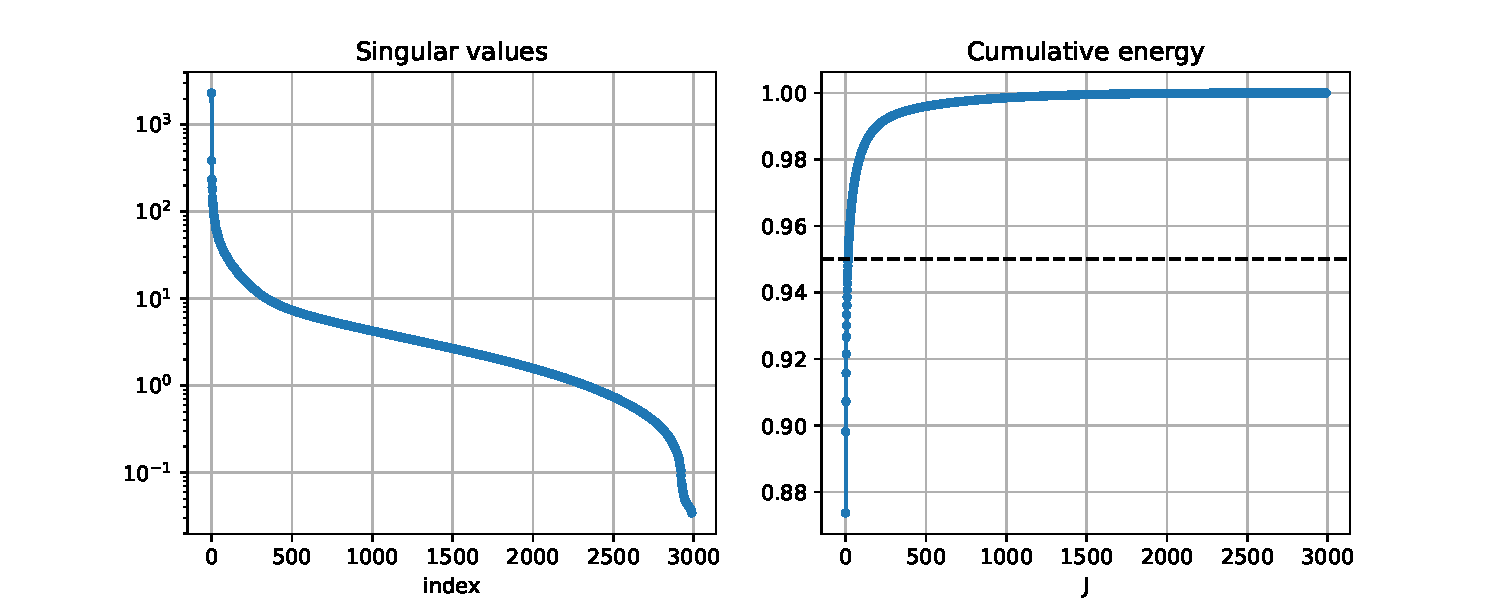
\includegraphics[width=\linewidth]{images/sing_value_to_energy.pdf}
		\caption{Relação entre os valores singulares e a energia dos mesmos.}
		\label{fig:mse_wave}
	\end{figure}
	
	Assim, partimos para a adição de ruído, que vai depender do truncamento J selecionado a partir do perfil de energia e da própria matriz AWGN. Podemos observar o comportamento do ruído controlado pela SNR com o truncamento pelo Mean Square Error(MSE), em contraste com o número $J$, como mostrado na figura \ref{fig:mse_noise}: 
	
	\begin{figure}[!h]
		\centering
		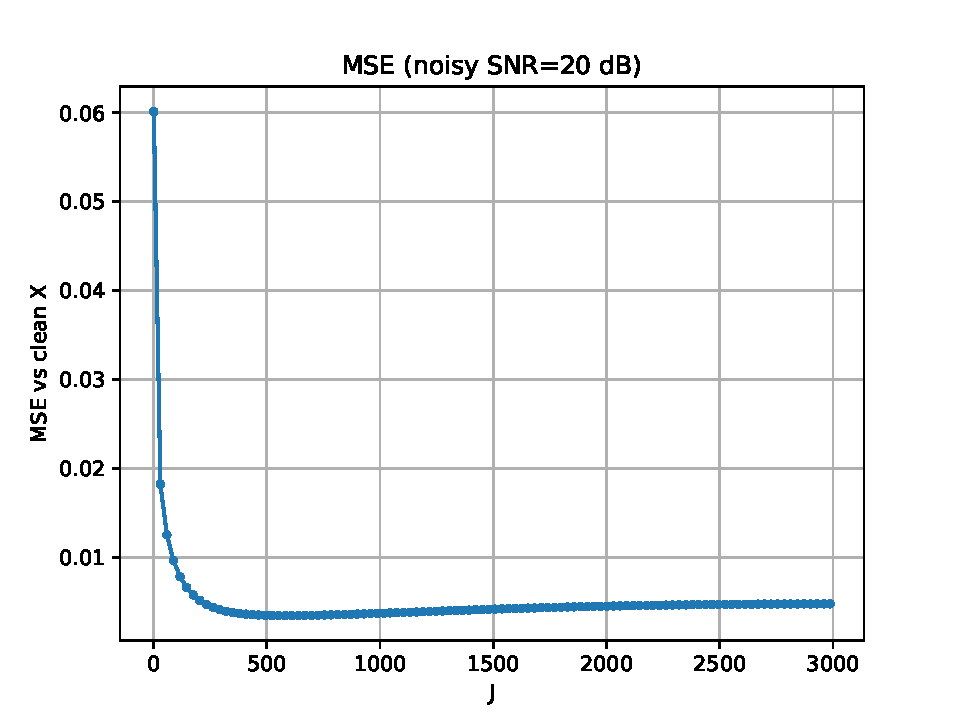
\includegraphics[width=0.9\linewidth]{images/mse_snr_com_ruido.pdf}
		\caption{MSE da SNR de acordo com a imagem limpa, relacionado ao valor de J.}
		\label{fig:mse_noise}
	\end{figure}
	
	Obtemos, como resultado final, a imagem restaurada com ruído, na Figura \ref{fig:wave_noise}:
	
	\begin{figure}[!h]
		\centering
		\includegraphics[width=0.7\linewidth]{images/noisy_recon_J.pdf}
		\caption{Imagem reconstruída com ruído, demonstrando a capacidade de redução de ruído da SVD}
		\label{fig:wave_noise}
	\end{figure}
	
	Segue abaixo o código utilizado para gerar as figuras  relativos ao problema 01: 
	\newpage
	\begin{lstlisting}
		import numpy as np
		import matplotlib.pyplot as plt
		from imageio import imread, imwrite
		from numpy.linalg import svd
		from skimage import img_as_float, img_as_ubyte
		
		img = img_as_float(imread('svd.jpg', pilmode='L'))  
		X = np.array(img, dtype=float)
		M, N = X.shape
		
		U, s, Vt = svd(X, full_matrices=False) 
		energy = s**2
		cum_energy = np.cumsum(energy) / np.sum(energy)
		
		
		plt.figure(figsize=(10,4))
		plt.subplot(1,2,1)
		plt.semilogy(s, '.-') 
		plt.title('Singular values') 
		plt.xlabel('index')
		plt.grid(True)
		plt.subplot(1,2,2)
		plt.plot(cum_energy, '.-')
		plt.title('Cumulative energy')
		plt.xlabel('J')
		plt.axhline(0.95, color='k', linestyle='--')
		plt.grid(True); plt.show()
		
		threshold = 0.99
		J = np.searchsorted(cum_energy, threshold) + 1
		def reconstruct_from_svd(U, s, Vt, J):
		return (U[:, :J] * s[:J]) @ Vt[:J, :]
		
		XJ = reconstruct_from_svd(U, s, Vt, J)
		
		imwrite('recon_J.pdf', img_as_ubyte(np.clip(XJ,0,1)))
		
		def add_awgn(X, snr_db):
		M, N = X.shape
		signal_energy = np.linalg.norm(X, 'fro')**2 
		snr_linear = 10**(snr_db/10.0)
		sigma = np.sqrt(signal_energy / (M*N*snr_linear))
		Z = np.random.normal(scale=sigma, size=X.shape)
		return X + Z, sigma
		
		snr_db = 20
		Y, sigma = add_awgn(X, snr_db)
		
		U_y, s_y, Vt_y = svd(Y, full_matrices=False)
		cum_energy_y = np.cumsum(s_y**2) / np.sum(s_y**2)
		
		
		def mse(A,B): return np.mean((A-B)**2)
		
		Js = list(range(1, min(M,N)+1, max(1, min(M,N)//100)))
		mses = []
		for j in Js:
		Yj = reconstruct_from_svd(U_y, s_y, Vt_y, j)
		mses.append(mse(X, Yj))
		
		plt.figure()
		plt.plot(Js, mses, '.-')
		plt.xlabel('J'); plt.ylabel('MSE vs clean X');
		plt.title(f'MSE (noisy SNR={snr_db} dB)')
		plt.grid(True); plt.show()
		
		J_example = J
		YJ_example = reconstruct_from_svd(U_y, s_y, Vt_y, J_example)
		imwrite('noisy_recon_J.pdf', img_as_ubyte(np.clip(YJ_example,0,1)))
		
		
		def psnr(X, Xhat, maxval=1.0):
		msev = np.mean((X - Xhat)**2)
		if msev == 0: return float('inf')
		return 10*np.log10(maxval**2 / msev)
		
	\end{lstlisting}
	
	Problema 2: Estimativa de Rank para Decomposição Tensorial
	
	Em muitas aplicações de processamento de sinais, especialmente aquelas que envolvem dados multidimensionais, tensores são usados para representar os dados. Um problema comum é estimar o posto de um tensor, que é o menor número de componentes necessários para representá-lo com precisão. O algoritmo de Mínimos Quadrados Alternados (ALS) é um método popular para decompor tensores em suas partes constituintes, mas seu desempenho depende fortemente da estimativa correta do posto do tensor.
	
	O algoritmo ALS funciona otimizando iterativamente cada componente da decomposição tensorial, mantendo os outros componentes fixos. O algoritmo requer uma estimativa inicial para o posto do tensor e, se essa estimativa estiver incorreta, a qualidade da decomposição pode ser significativamente prejudicada.
	
	Para estudar o impacto da estimativa de posto no algoritmo ALS, realizamos experimentos de Monte Carlo. Em cada experimento, geramos um tensor com ruído e aplicamos o algoritmo ALS com diferentes classificações estimadas. Em seguida, medimos o erro de reconstrução, que quantifica o quão bem o tensor decomposto corresponde ao tensor original sem ruído. Repetindo esse processo várias vezes, podemos observar o desempenho médio do algoritmo ALS para cada classificação estimada.
	
	Quando a classificação estimada é muito baixa (subestimação), o algoritmo ALS não consegue capturar todos os componentes importantes do tensor, levando a um alto erro de reconstrução. Isso ocorre porque o modelo é muito simples para representar a estrutura de dados subjacente. Por outro lado, quando a classificação estimada é muito alta (superestimação), o algoritmo ALS pode capturar ruído como se fosse parte do sinal, levando ao sobreajuste. Isso também resulta em um erro de reconstrução maior, embora o aumento geralmente seja menos severo do que com a subestimação.
	
	O desempenho ideal é alcançado quando a classificação estimada corresponde à classificação real do tensor. Nesse ponto, o algoritmo ALS consegue representar o tensor com precisão, sem sobreajuste ou subajuste. A classificação verdadeira pode frequentemente ser identificada observando-se o ponto em que o erro de reconstrução para de diminuir significativamente à medida que a classificação estimada aumenta.
	
	Em aplicações práticas, é crucial validar a classificação escolhida usando técnicas como validação cruzada ou análise de consistência central. Esses métodos ajudam a garantir que a classificação estimada não seja excessivamente influenciada por ruído ou outros artefatos nos dados.
	
	Depois de executar o código, obtemos como resultado: 
	
	\begin{figure}[h!]
		\centering
		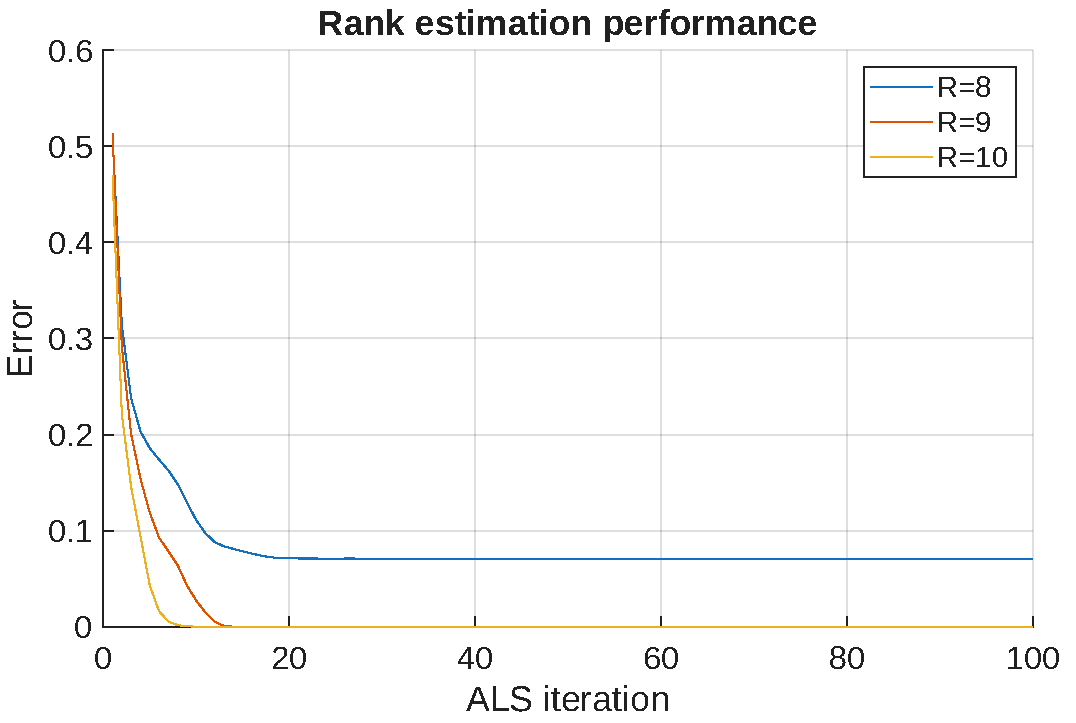
\includegraphics[width=0.9\linewidth]{images/ALS_rank_estimation_cropped.pdf}
		\caption{Estimação do erro de aproximação de ranking para R=$\{8,9,10\}$.}
		\label{fig:ALS}
	\end{figure}
	
	Segue abaixo o código utilizado para gerar a figura \ref{fig:ALS} (solução do problema 02):
	\begin{lstlisting}
		import numpy as np
		import scipy.io as sio
		import mat73
		import matplotlib.pyplot as plt
		
		mat_data = mat73.loadmat('ten_H.mat')
		H_clean = mat_data['ten_H']
		
		# parametros dados na questao
		R_candidates = np.arange(1, 10)
		nMC = 1000
		SNR_dB = 20
		maxIter = 100
		
		mean_final_err = np.zeros(len(R_candidates))
		std_final_err  = np.zeros(len(R_candidates))
		mean_iter_err  = []
		
		def add_noise_to_tensor(H_clean, SNR_dB):
		signal_energy = np.linalg.norm(H_clean)**2
		snr_linear = 10**(SNR_dB/10)
		sigma = np.sqrt(signal_energy / (H_clean.size * snr_linear))
		noise = sigma * np.random.randn(*H_clean.shape)
		return H_clean + noise
		
		for idx, Rhat in enumerate(R_candidates):
		final_errs = np.zeros(nMC)
		iter_traces = np.zeros((nMC, maxIter))
		
		for mc in range(nMC):
		H_noisy = add_noise_to_tensor(H_clean, SNR_dB)
		y, final_err = ALS_estimation(H_noisy, Rhat, SNR_dB)
		final_errs[mc] = final_err
		
		L = min(len(y), maxIter)
		iter_traces[mc, :L] = y[:L]
		if L < maxIter:
		iter_traces[mc, L:] = y[-1]
		
		mean_final_err[idx] = np.mean(final_errs)
		std_final_err[idx] = np.std(final_errs)
		mean_iter_err.append(np.mean(iter_traces, axis=0))
		
		plt.figure()
		to_plot = [1, R_candidates[len(R_candidates)//2], R_candidates[-1]]
		for R in to_plot:
		idx = np.where(R_candidates == R)[0][0]
		plt.plot(mean_iter_err[idx], lw=1.2, label=fr'$\hat{{R}}$={R}')
		
		plt.legend()
		plt.xlabel('ALS iteration')
		plt.ylabel('Mean error')
		plt.grid(True)
		plt.title('Mean ALS iteration error for selected $\hat{R}$')
		plt.show()
	\end{lstlisting}
	
	\section{Homework 00 multilinear}
	
	Geramos aleatoriamente A e B em uma simulação de monte carlo.
	
	
	
	% \section{Homework 09 multilinear}
	
	% A ideia é decompor um tensor de ordem superior (neste caso, um tensor de terceira ordem $\mathcal{X}$) em uma soma de $R$ componentes de rank-1. Cada componente de rank-1 é o produto externo de $R$ vetores, ou seja o rank do tensor.
	
	% Onde $\mathbf{a}_r$, $\mathbf{b}_r$ e $\mathbf{c}_r$ são os $r$-ésimos vetores das matrizes fatoriais A, B e C, respectivamente, e $\circ$ denota o produto externo. Na prática, isso é equivalente a encontrar as matrizes fatoriais A, B e C.
	
\end{document}
